% \newcommand\fnote[1]{\captionsetup{font=small}\caption*{#1}}

% % \begin{figure*}[!t]
% % \begin{minipage}{.5\linewidth}
% % \centering
% %         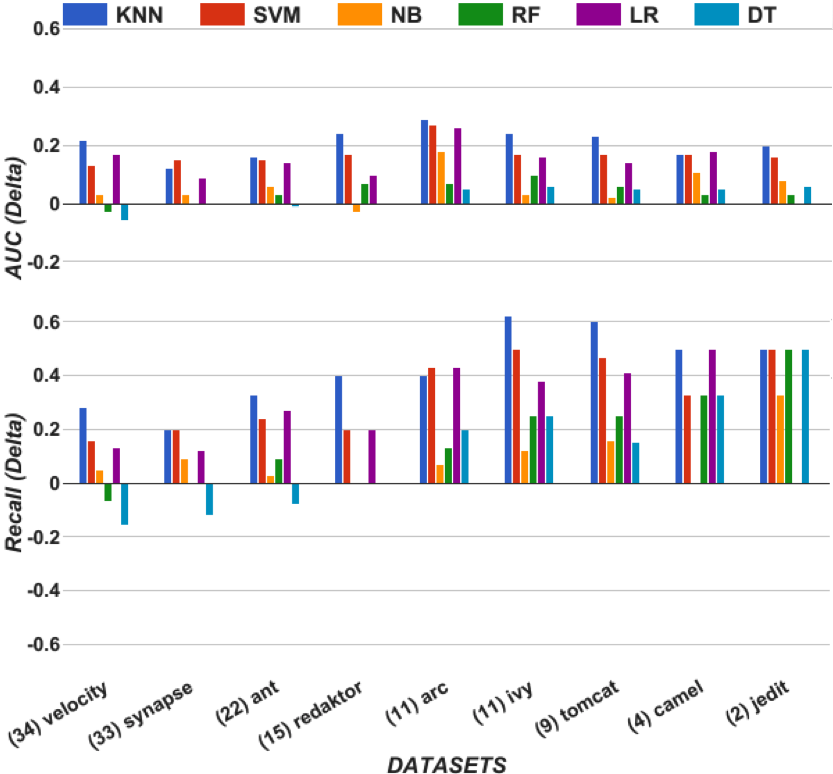
\includegraphics[width=.95\linewidth]{./fig/AUC_recall_untuned.png}
% %     \end{minipage}%
% % \begin{minipage}{.5\linewidth}
% %         \centering
% %         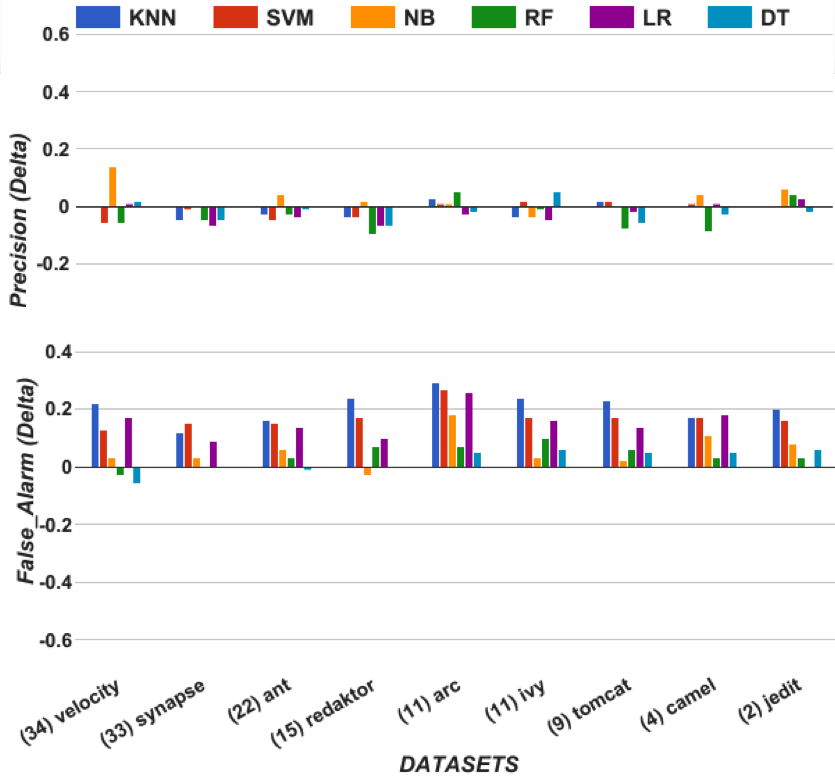
\includegraphics[width=.95\linewidth]{./fig/prec_pf_untuned.png}
% %     \end{minipage}%
% %     \caption{SMOTE improvement over No-SMOTE. Legends represent the classifiers mentioned in \tion{classes}}
% %     \vspace{-11pt}
% %     \fnote{For subfigures (AUC, Recall and Precision): larger y-values are {\em better}, if the y-value goes {\em negative}, then the corresponding learner trained on SMOTE data performs {\em worse} than learner learnt on raw data. For false alarms, the plot must be interpreted differently: larger y-values are {\em worse}, if the y-value goes {\em positive}, then the corresponding learner trained on SMOTE data performs {\em worse} than learner learnt on raw data. The corresponding percentage of minority class (in this case, defective class) is written beside each dataset.}
% %     \label{fig:untuned}
% % \end{figure*}


% \begin{figure*}[!t]
%     \centering
%     \begin{minipage}{.33\textwidth}
%     \centering
%         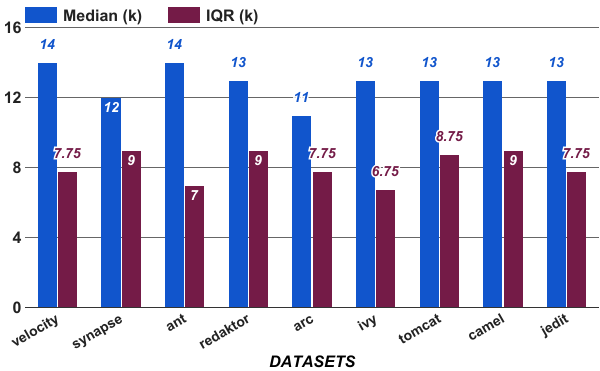
\includegraphics[width=.95\linewidth]{./fig/k.png}
%         {\bf Figure~\ref{fig:para}a:} Tuned values for $k$. Note that the default value for $k$ is $k=2$.
%     \end{minipage}%
%     \begin{minipage}{.33\textwidth}
%     \centering
%         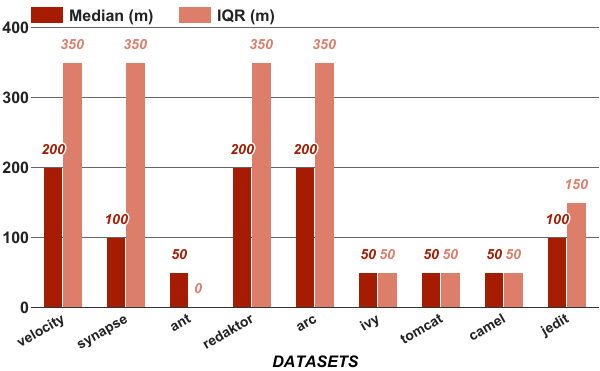
\includegraphics[width=.95\linewidth]{./fig/m.png}
%         {\bf Figure~\ref{fig:para}b:} Tuned values for $m$.
%         Note that the default value for  $m$ is $m=100$.
%     \end{minipage}
%     \begin{minipage}{.33\textwidth}
%     \centering
%         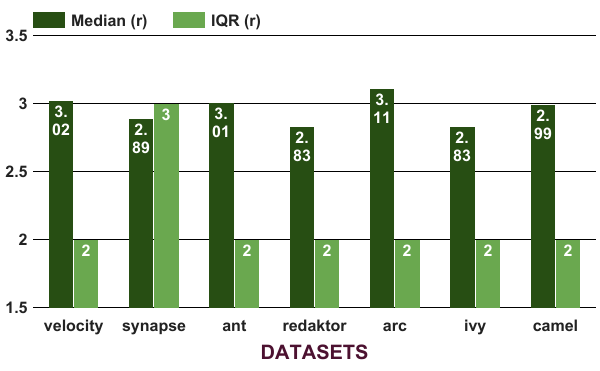
\includegraphics[width=.95\linewidth]{./fig/r.png}
%         {\bf Figure~\ref{fig:para}c:} Tuned values for $r$.
%         Note that the default value for $r$ is $r=3$.
%     \end{minipage}
%     \caption{Datasets vs Parameter Variation}
%     \label{fig:para}
% \vspace{-0.4cm}
% \end{figure*}
   

% \section{Results}
% \label{sect:results}

% Our results are organized around the three
% research questions introducted in the introduction
% to this paper.

%  \subsection{RQ1: Are the default ``off-the-shelf'' parameters for SMOTE appropriate for all
%  data sets?}
 
 
%  As discussed above, the default parameters for
%  SMOTE are $k,m,r = 5,100,2$.
%   Figure~\ref{fig:para} shows the range of parameters
%  found by SMOTE across  nine data sets for the 25 repeats of our cross-validation procedure.
%  All the results in this figure are {\em within-measure assessment} results; i.e.
%  here, we SMOTUNED trains of some performance measure and then we only collect performance for that performance measure in the test set.
 
 
%  In  Figure~\ref{fig:para}, {\em median} is the 50th percentile
%  value and {\em IQR} is the (75-25)th percentile
%  (IQR is a non-parametric analgoue of variance).
%  As can be seen in Figure~\ref{fig:para}, most of the learned parameter are far from the default values:
%  \bi
%  \item 
%  Median $k$ value was never less than 11;
%  \item
%  Median m value of often twice or half the default value used in SMOTE;
%  \item
%  The $r$ value used in the distance function was never 2. Rather, it was usually 3.
%  \ei
%  Hence,  our answer to {\bf RQ1} is ``no'': the use of off-the-shelf SMOTE should be deprecated. 
   



% \subsection {RQ2: What are there benefit in tuning the default parameters of SMOTE for each new data set?}

% Figure~\ref{fig:tuned} shows the performance delta of the {\em within-measure assessment rig}.
% Recall that when this rig applies SMOTUNED, it optimizes for performance measure
% \[M_i \in \{ 
% \mathit{recall},
% \mathit{precision}, 
% \mathit{false\; alarm},
% \mathit{AUC}
% \}
% \]
% after which it uses the {\em same} performance measure
% when processing test data.
% As shown in Figure~\ref{fig:tuned}, 
% SMOTUNED achieves large AUC and recall improvements
% without
%  damaging precision and  with only minimal changes
%  to false alarms. Special note should be take of the  AUC improvements- these are the largest improvements
%  we have yet seen, for any prior treatment of defect prediction data.

% Figure~\ref{fig:stats} offers a statistical 

 
%  false alarms and with only minimal changes to false alar,s.
% The first thing to note in are the very large improvements in AUC and recall and the 
% very small changes to precision and false alarm:

% \bi
% \item The AUC delta results are some of the largest we have ever seen, for any treatment, in any defect prediction paper.
% \item The precision delta results are particularly small;
% i.e. 


% That is, Figure~\ref{fig:tuned} offers much evidence that SMOTUNED is useful


%   \subsection{RQ2: In terms of the performance of defect predictors, are there benefit in tuning the default parameters of SMOTE for each new data set?}

%  \begin{lesson}For defect data, {\sma} has adverse effect on 
%  precision, modest improvements for AUC (pf, recall) and large improvements in recall.
%  \end{lesson}


% \begin{figure*}[!t]
% \begin{minipage}{.5\linewidth}
% \centering
%         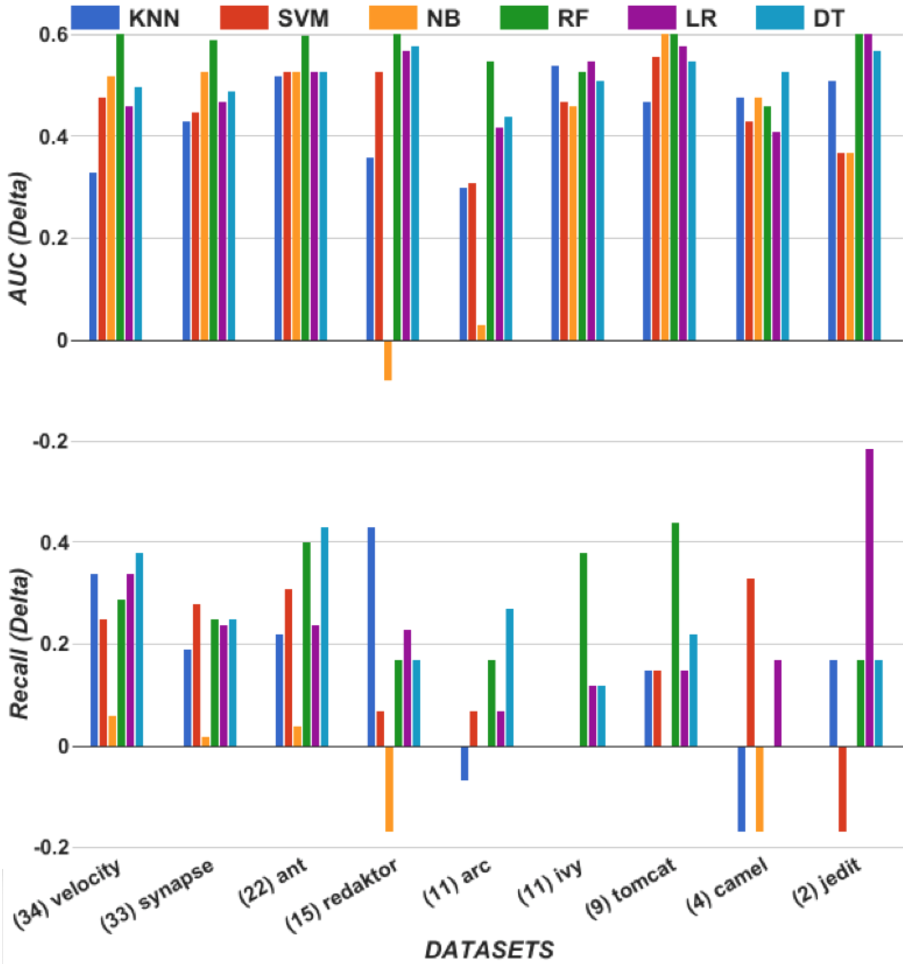
\includegraphics[width=.95\linewidth]{./fig/AUC_recall_tuned.png}
%     \end{minipage}%
% \begin{minipage}{.5\linewidth}
%         \centering
%         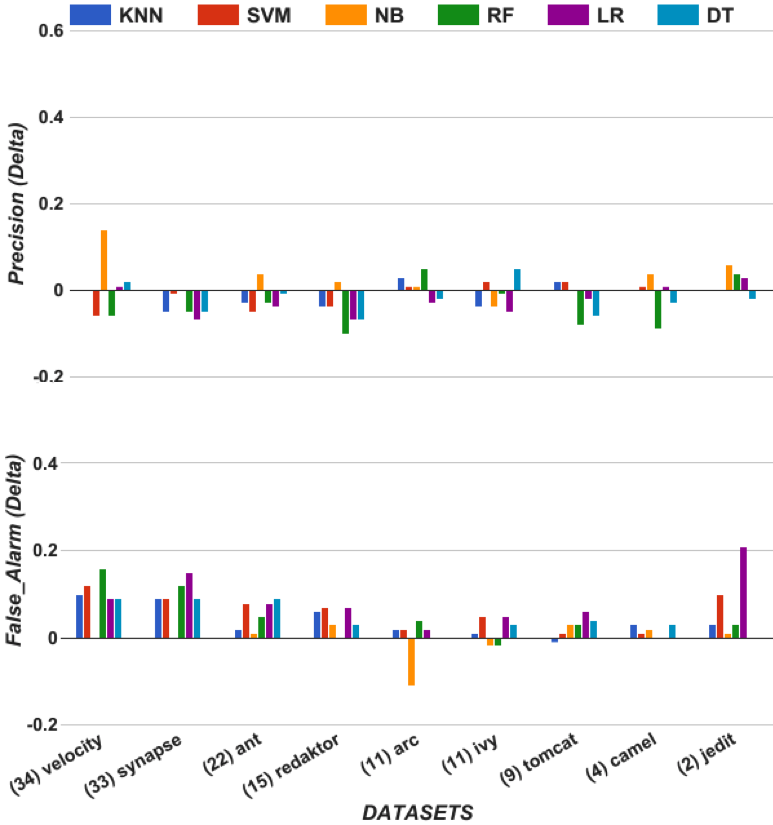
\includegraphics[width=.95\linewidth]{./fig/prec_pf_tuned.png}
%     \end{minipage}%
    
%     \caption{SMOTUNED improvement over SMOTE. Legends represent the classifiers mentioned in \tion{classes}.}
%     \vspace{-10pt}
%     \fnote{For subfigures (AUC, Recall and Precision): larger y-values are {\em better}, if the y-value goes {\em negative}, then the corresponding learner trained on SMOTUNED data performs {\em worse} than learner learnt on SMOTE data. For false alarms, the plot must be interpreted differently: larger y-values are {\em worse}, if the y-value goes {\em positive}, then the corresponding learner trained on SMOTUNED data performs {\em worse} than learner learnt on SMOTE data. The corresponding percentage of minority class (in this case, defective class) is written beside each dataset.}
%     \label{fig:tuned}
% \end{figure*}

% \begin{figure*}[!htbp]
% \begin{minipage}{.5\linewidth}
% \centering
%         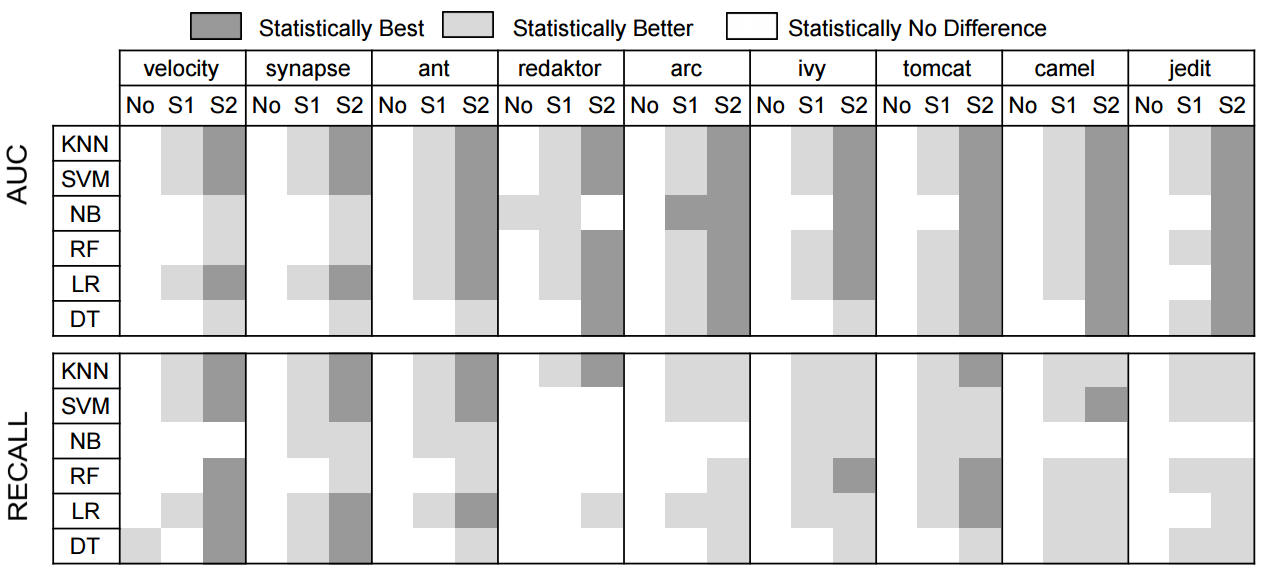
\includegraphics[width=.9\linewidth]{./fig/AUC_recall.png}
%             \end{minipage}%
% \begin{minipage}{.5\linewidth}
%         \centering
%         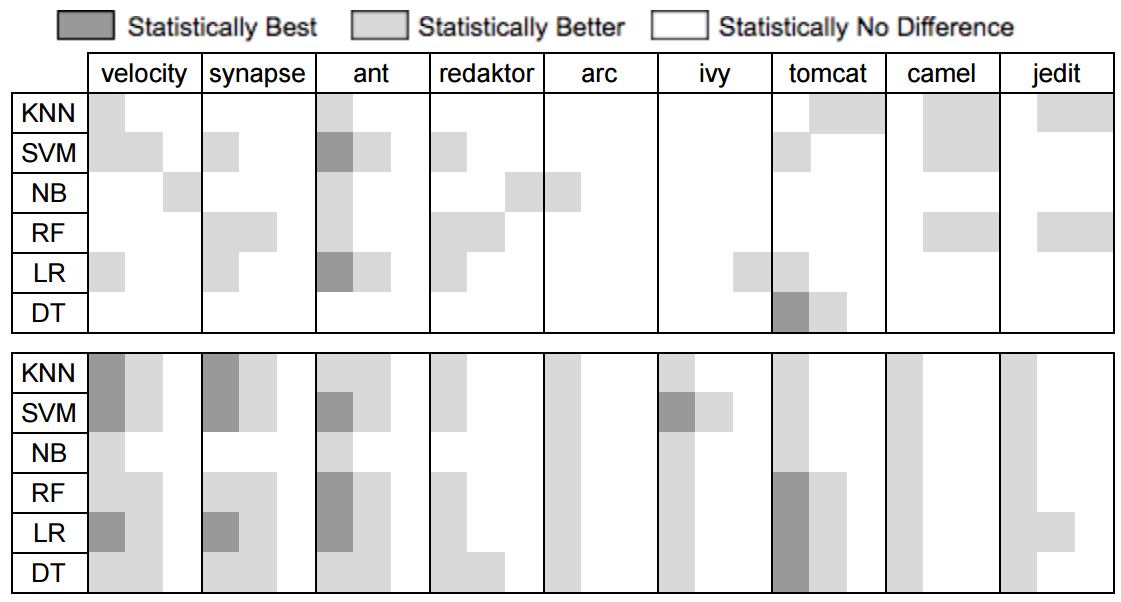
\includegraphics[width=.9\linewidth]{./fig/prec_pf.png}
%     \end{minipage}%
%     \caption{Scott Knott analysis of No-SMOTE, SMOTE and SMOTUNED. The column headers are denoted as No for No-SMOTE, S1 for SMOTE and S2 for SMOTUNED. $(\ast)$ Mark represents the best learner combined with its techniques.}
%     \label{fig:stats}
% \vspace{-0.2cm}
% \end{figure*}

%  \textbf{RQ2}: \textbf{Can {\smb} achieve better results?} 
 
%  \begin{lesson}For defect data, {\smb}  
%  offered    improvements over {\sma} for recall
%  and dramatic improvements for AUC (pf, recall).
%  \end{lesson}
 
%  \textbf{RQ3}: \textbf{Does hyperparameter optimization lead to different optimal configurations for different datasets?} 
 
%  \begin{lesson}Yes. DE finds different ``best'' parameter settings for {\sma} on different datasets.
%  \end{lesson}
%   This is an important result
%   since it means
%   reusing tunings suggested  by  any other  previous study  for a dataset different from the one under study is \underline{{\em not}} recommended. Instead,  it is better to
%       use automatic tuning  methods  to find the best tuning parameters for the 
%       under study dataset.
      
%       Note that
%  before we demand that tuning should be a
%  standard for all analytics task,
%  we must assess the practicality of that
%  proposal. This leads to the next question:
 
%   \textbf{RQ4}: \textbf{Is tuning 
%   impractically
%   slow?} 
 
%  \begin{lesson}Tuning using DE makes training runtimes about twenty times slower, but given
%  the large performance improvements,
%  the extra effort is justifiable. \end{lesson}
 
 



% \subsection{\textbf{RQ1: Is standard ``off-the-shelf'' SMOTE preprocessing method useful for defect prediction?}}

% Figure~\ref{fig:stats} shows Scott-Knott analysis of No-Smote, SMOTE and SMOTUNED. Each subfigure shows the 4 different evaluation measures (mentioned in \tion{measure}) compared with 6 learners (mentioned in \tion{classes}). The columns are sorted in the decreasing percentage of defective classes from left to right.

% For many of the results in Figure~\ref{fig:stats}, the changes
% resulting from applying SMOTE are very modest. There are improvements in AUC and recall with SMOTE over No-Smote but the improvements are not big as compared with SMOTUNED.

% The two consistent exceptions to that pattern are:
% \bi
% \item 
% SMOTE is not preferred when we can achieve better performance with SMOTUNED
% \item 
% Occasionally, SMOTE leads to poor performance in precision and false alarm but in many cases, they are not statistically significant different as shown in Figure~\ref{fig:stats}.  
% \ei

% We are not seeing any improvement in precision nor decrement in false alarm, the reason behind this is its maths. Zhang's~\cite{menzies2007problems} equation as given by Zhang can be rearranged to:
% \[
%   \mathit{pf}=  \frac{pos}{neg} *\frac{1-\mathit{prec}}{\mathit{prec}}* \mathit{pd}\]

% Pos and neg in the equation represents the imbalance ratio among the data samples. When we consider, pos to neg ratio and $prec$ constant, we are seeing there is direct relation between $pf$ and $pd$. So if pd is improved, we are bound to see improvement in pf. AUC is used to balance out this relation between pf and pd recommending to have higher AUC. On the other hand with prec, pf has indirect relation and since pf is increasing which is making prec improvements negligible.

% %  False positives (from Figure~\ref{fig:cmatrix}) do not get reduced after applying SMOTE. SMOTE generates synthetic examples within defective data samples and its neighbors making more denser region for positive samples. So if there are any actual negative samples surrounding these denser regions will now get wrongly classified as positive by learners. 

% % Based on these results,  we can best recommend SMOTE when:
% % \bi
% % \item Trying to improve recall
% % for imbalanaced datasets;
% % \item
% % Using NB or Random Forests.
% % \ei

% % For SMOTUNED improvement over SMOTE (figure~\ref{fig:tuned}), AUC values are shown in subfigure~\ref{fig:tuned}a. Redaktor dataset is selected from X-axis, and yellow bar represents NB which corresponds to about $-0.08$ AUC value. This denotes that NB performed worse by tuning the parameters of SMOTE. The original parameter settings of SMOTE worked the best. On the other hand for the same dataset, KNN (which is represented in dark blue bar) shows the AUC value of $0.35$. This shows KNN outperformed the ``off-the-shelf'' SMOTE when tuned using DE.



% % By looking at the results of AUC from figure~\ref{fig:untuned}a, only 4 bars are negative, and rest all the remaining 50 bars (in total 9 datasets with 6 learners in each) have  positive effect by using SMOTE as a preprocessing method. We are seeing a maximum improvement of about 30\%. These improvements are quite modest as to ignore the importance of SMOTE.

% % Results for precision (in figure~\ref{fig:untuned}b), are not much interesting, but the decrease in precision value is not that arduous except for the redaktor dataset. Though we will not recommend using SMOTE whenever we want higher precision value. Since precision is decreased using SMOTE, it was expected to have increased false alarm \cite{menzies2007problems} and the same is observed from figure~\ref{fig:untuned}d. There is an increase in error among false positives but the increase is very minimal.

% % As for recall (figure~\ref{fig:untuned}c), only 4 bars are negative, and rest all the remaining 50 bars (in total 9 datasets with 6 learners in each) have positive effect by using SMOTE. We are seeing a maximum improvement of about 60\%. These improvements are quite steep as to ignore the importance of SMOTE at any point for any learner. It is also observed that performance keeps increasing as target class becomes more minor and minor. This is what was expected after applying SMOTE to imbalance datasets.

% \noindent
% Summarizing the above:
% \begin{lesson1}
% We recommend SMOTE for improving recall, but SMOTE can,
% sometimes, adversely affect
% precision.
% \end{lesson1}


% \subsection{\textbf{RQ2: Can SMOTUNED achieve better results?}}

% Figure~\ref{fig:tuned} shows the results
% after applying SMOTUNED. The
% plot shows the {\em delta} between
% the results obtained by SMOTUNED over SMOTE.

% For subfigures (AUC, Recall and Precision):
% \bi
% \item 
% {\em Larger} y-values
% are {\em better} 
% \item
% If the y-value goes {\em negative}, then the corresponding learner trained on SMOTUNED data is {\em worse} than learner learnt on SMOTE data respectively. 
% \ei
% For the false alarms, the
% plots must be interpreted differently:
% \bi
% \item
% {\em Larger} y-values are {\em worse};
% \item
% If the y-value goes {\em positive} then the corresponding learner trained on SMOTUNED data is {\em worse} than learner learnt on SMOTE data respectively.
% \ei

% The benefit of SMOTUNED's tunings is clearly evident in the AUC results of  Figure~\ref{fig:tuned}a:
% all learners show large performance improvements. And from the Scott-Knott test shown in Figure~\ref{fig:stats}, SMOTUNED always have significantly best results for AUC. For recall, in most learners either SMOTE or SMOTUNED are significantly the same, or SMOTUNED performed better. 
% Better yet,  as
% shown in
% Figure~\ref{fig:stats}, for precision and false alarm, SMOTUNED does
% not adversely effect false alarm and precision as most of the times No-SMOTE, SMOTE, and SMOTUNED are significantly the same.


% At first glance, SMOTUNED's effects on recall seem strange since they are
% {\em better} for the more balanced left-hand-side datasets of
% Figure~\ref{fig:tuned}c.  But recall from the above that SMOTE had less
% of an effect on those left-hand-side datasets. That is, what we are seeing
% here is that:
% \bi
% \item
% SMOTUNED works often as well as SMOTE for imbalanced datasets;
% \item
% SMOTUNED offers additional benefits for datasets that are not greatly
% imbalanced.
% \ei


% % results are dramat
% % Now when we look at the results of AUC from figure~\ref{fig:tuned}a, only 1 bar is negative, and rest all the remaining 53 bars (in total 9 datasets with 6 learners in each) have  positive effect after when we tune the parameters of SMOTE. We are seeing a maximum improvement of about 70\% and on an average 50\% for each learner in all datasets. These improvements are quite steep in nature and just to remind you that these results are improvement over SMOTE. If we combine the results, then we can surely say to tune the parameters of SMOTE and train using any learner, we will get atleast 100\% improvement in most cases.

% % We are seeing the similar trend of results for precision (in figure~\ref{fig:tuned}b), just like in Figure~\ref{fig:untuned}b, that even after tuning for precision, we are not seeing much improvement. Though we definitely improved precision slightly than SMOTE but the increment is not that large to recommend SMOTUNED or SMOTE. And even after trying to minimise the false alarm (figure~\ref{fig:tuned}d) value, DE could not find a good parameter setting.

% % As for recall (figure~\ref{fig:untuned}c), only 5 bars are negative, and rest all the remaining 49 bars (in total 9 datasets with 6 learners in each) have either positive effect or no effect after tuning. We are seeing a maximum improvement of about 65\% but the average improvement is close to 15\% for each classifiers in all datasets. But these improvements combined with SMOTE suggest that we should always tune SMOTE whenever the goal is to achieve higher recall.

% In summary:

% \begin{lesson1}
%     For defect data, SMOTUNED  
%  offers   some  improvements over SMOTE for recall
%  and dramatic improvements for AUC (pf, recall).
%  The effects on precision and false alarm are similar to SMOTE.
% \end{lesson1}

% %Based on these results, we strongly recommend SMOTUNED for handling not just unbalanced datasets but, in fact, for all datasets.

% \subsection{\textbf{RQ3: Does hyperparameter optimization lead to different optimal configurations for different datasets?}}

% Figure \ref{fig:para} represents the parameter variations when we tuned to maximize the recall. These parameter settings are found by each learner for that dataset.
% On display in each set of vertical bars are
% the median values generated across 25 evaluations.
% Also, shown are
% the inter-quartile range (IQR) of those tunings (the IQR is the 75th-25th percentile values and is a non-parametric measure of variation
% around the median value). Note that in Figure \ref{fig:para}b, IQR=0 for  ant dataset where tuning always converged on the same final value. That shows that the maximum score of recall is reached when $m=50$. No other parameter setting found out to be useful by DE.

%   These figures
% show how tuning selects the different ranges  of
% parameters.
% Some of the above numbers are far from the standard values; e.g. Chawla et al.~\cite{chawla2002smote} recommend using $k=5$ neighbors yet in our datasets, best results were seen using $k \approx 13$. On other hand it was suggested to use $m=900$ by ~\cite{pears2014synthetic}.
% Clearly,
% best results from tuning
% vary with each dataset.

% Clearly:
% \begin{lesson1}
%     Yes. DE finds different ``best'' parameter settings for SMOTUNED on different datasets.
% \end{lesson1}
%  That is,  reusing tunings  suggested  by  any other  previous study  for any dataset is \underline{{\em not}} recommended. Instead,  it is better to
%       use  automatic  tuning  methods  to find the best tuning parameters for the current dataset.
      

% \begin{figure}[!htbp]
%   \captionsetup{justification=centering}
%   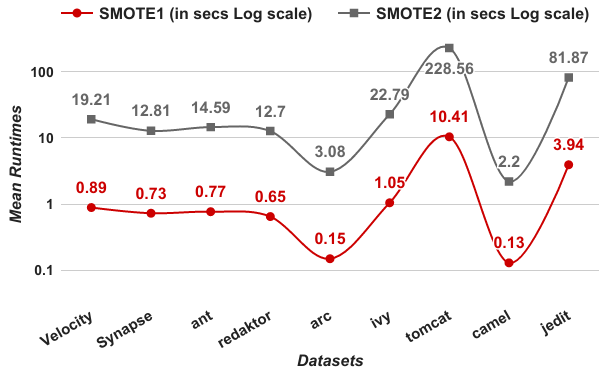
\includegraphics[width=\linewidth]{./fig/runtimes.png}
%   \caption{Datasets vs Runtimes. Note that the numbers
%   shown here at the total times for running six learners through a 5*5cross-validation. Hence, for mean
%   runtimes for one learner, {\em divide} these numbers by 6*5*5=150.}
%   \label{runtime}
% \vspace{-0.7cm}
% \end{figure}

% \begin{figure*}[!htbp]
% \begin{minipage}{.5\linewidth}
% \centering
%         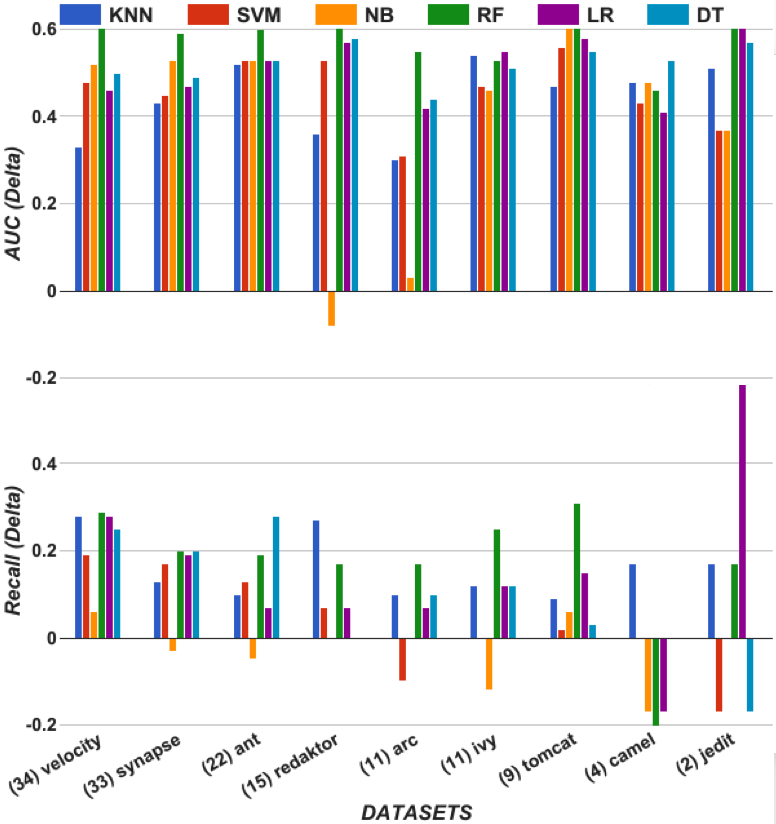
\includegraphics[width=.95\linewidth]{./fig/AUC_auc1.png}
%     \end{minipage}%
% \begin{minipage}{.5\linewidth}
%         \centering
%         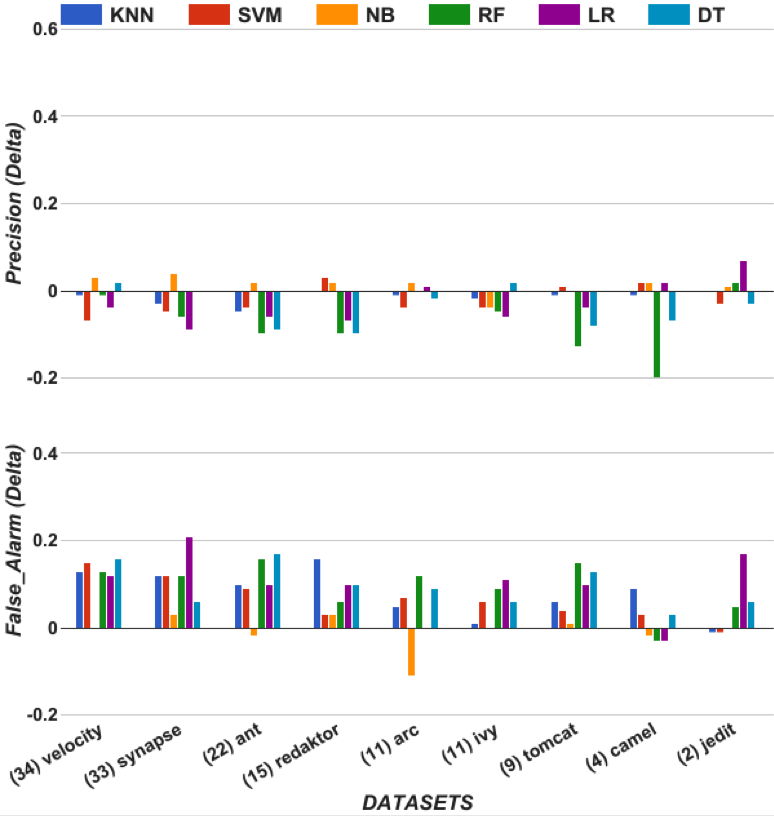
\includegraphics[width=.95\linewidth]{./fig/AUC_prec.png}
%     \end{minipage}%
    
%     \caption{SMOTUNED improvement over SMOTE when tuning goal is to maximize AUC.}
%     \vspace{-10pt}
%     \fnote{For subfigures (AUC, Recall and Precision): larger y-values are {\em better}, if the y-value goes {\em negative}, then the corresponding learner trained on SMOTUNED data performs {\em worse} than learner learnt on SMOTE data. For false alarms, the plot must be interpreted differently: larger y-values are {\em worse}, if the y-value goes {\em positive}, then the corresponding learner trained on SMOTUNED data performs {\em worse} than learner learnt on SMOTE data. The corresponding percentage of minority class (in this case, defective class) is written beside each dataset.}
%     \label{fig:auc}
% \vspace{-0.6cm}
% \end{figure*} 

% \subsection{\textbf{RQ4: Is tuning impractically slow?}}

% Search-based SE methods can be very slow. Wang et al.~\cite{wang2013searching} once needed 15
% years of CPU time to find and verify the tunings required for software
% clone detectors. Sayyad et al.~\cite{sayyad2013scalable} routinely used
% $10^6$ evaluations (or more) of their models in order to extract
% products from highly constrained product
% lines. Hence, before recommending any
% search-based method, it is wise to consider the runtime cost of that
% recommendation.


%  Figure~\ref{runtime} shows,  in circle and square markers, the
%   runtimes required to run SMOTE and SMOTUNED respectively and the numbers shown in the graph is an average over 6 learners.  The
%   longer runtimes (in square) include the times required for DE to find
%   the tunings and this is a disadvantage with SMOTUNED. Figure~\ref{runtime} shows SMOTE reporting all the measures in the shown time. On the other hand, here SMOTUNED reports runtimes when trying to maximize recall. If it has to provide all the other 3 measures as well, it would take 3 times more than the above number which is not recommended in a real world scenario. 
  
%   The work around would be is to try maximizing SMOTUNED for AUC tuning goal. AUC represents the area under the curve for pf (false alarm) and recall. When AUC improves, the heuristic is that false alarm must be getting lower and recall must be improving. And if false alarm is getting lower then precision is improving as well~\cite{menzies2007data}. We report results of AUC, Precision, Recall and False alarm in Figure~\ref{fig:auc} when we tried maximizing only AUC. We are seeing a similar conclusions as answered in our RQ2. 
  
%   This additional result shows that, tuning slows down the training by a factor of up to
%   twenty for 1 goal (which is very close to our theoretical prediction) but the improvements achieved are quite advantageous.

% \begin{lesson1}
%     Tuning with DE makes training about twenty times slower, but the improvements in performance with respect to AUC and recall justifies the extra time required for training.
% \end{lesson1}
